\section{Proposal-/Mask-Space Exploration}
\label{sec:proposal}

This section addresses \textbf{RQ3} by asking what the generated masks already contain. The proposal-/mask-space route treats frozen automatic masks as fragmented evidence rather than as final predictions. Given a frozen proposal bank, the route must decide which fragments belong together, which unions are contradictory, and whether a conservative core should be expanded. The key architectural point is simple: the proposal generator stays frozen throughout. What is learned is only the lightweight readout above that bank.

\begin{figure*}[t]
    \centering
    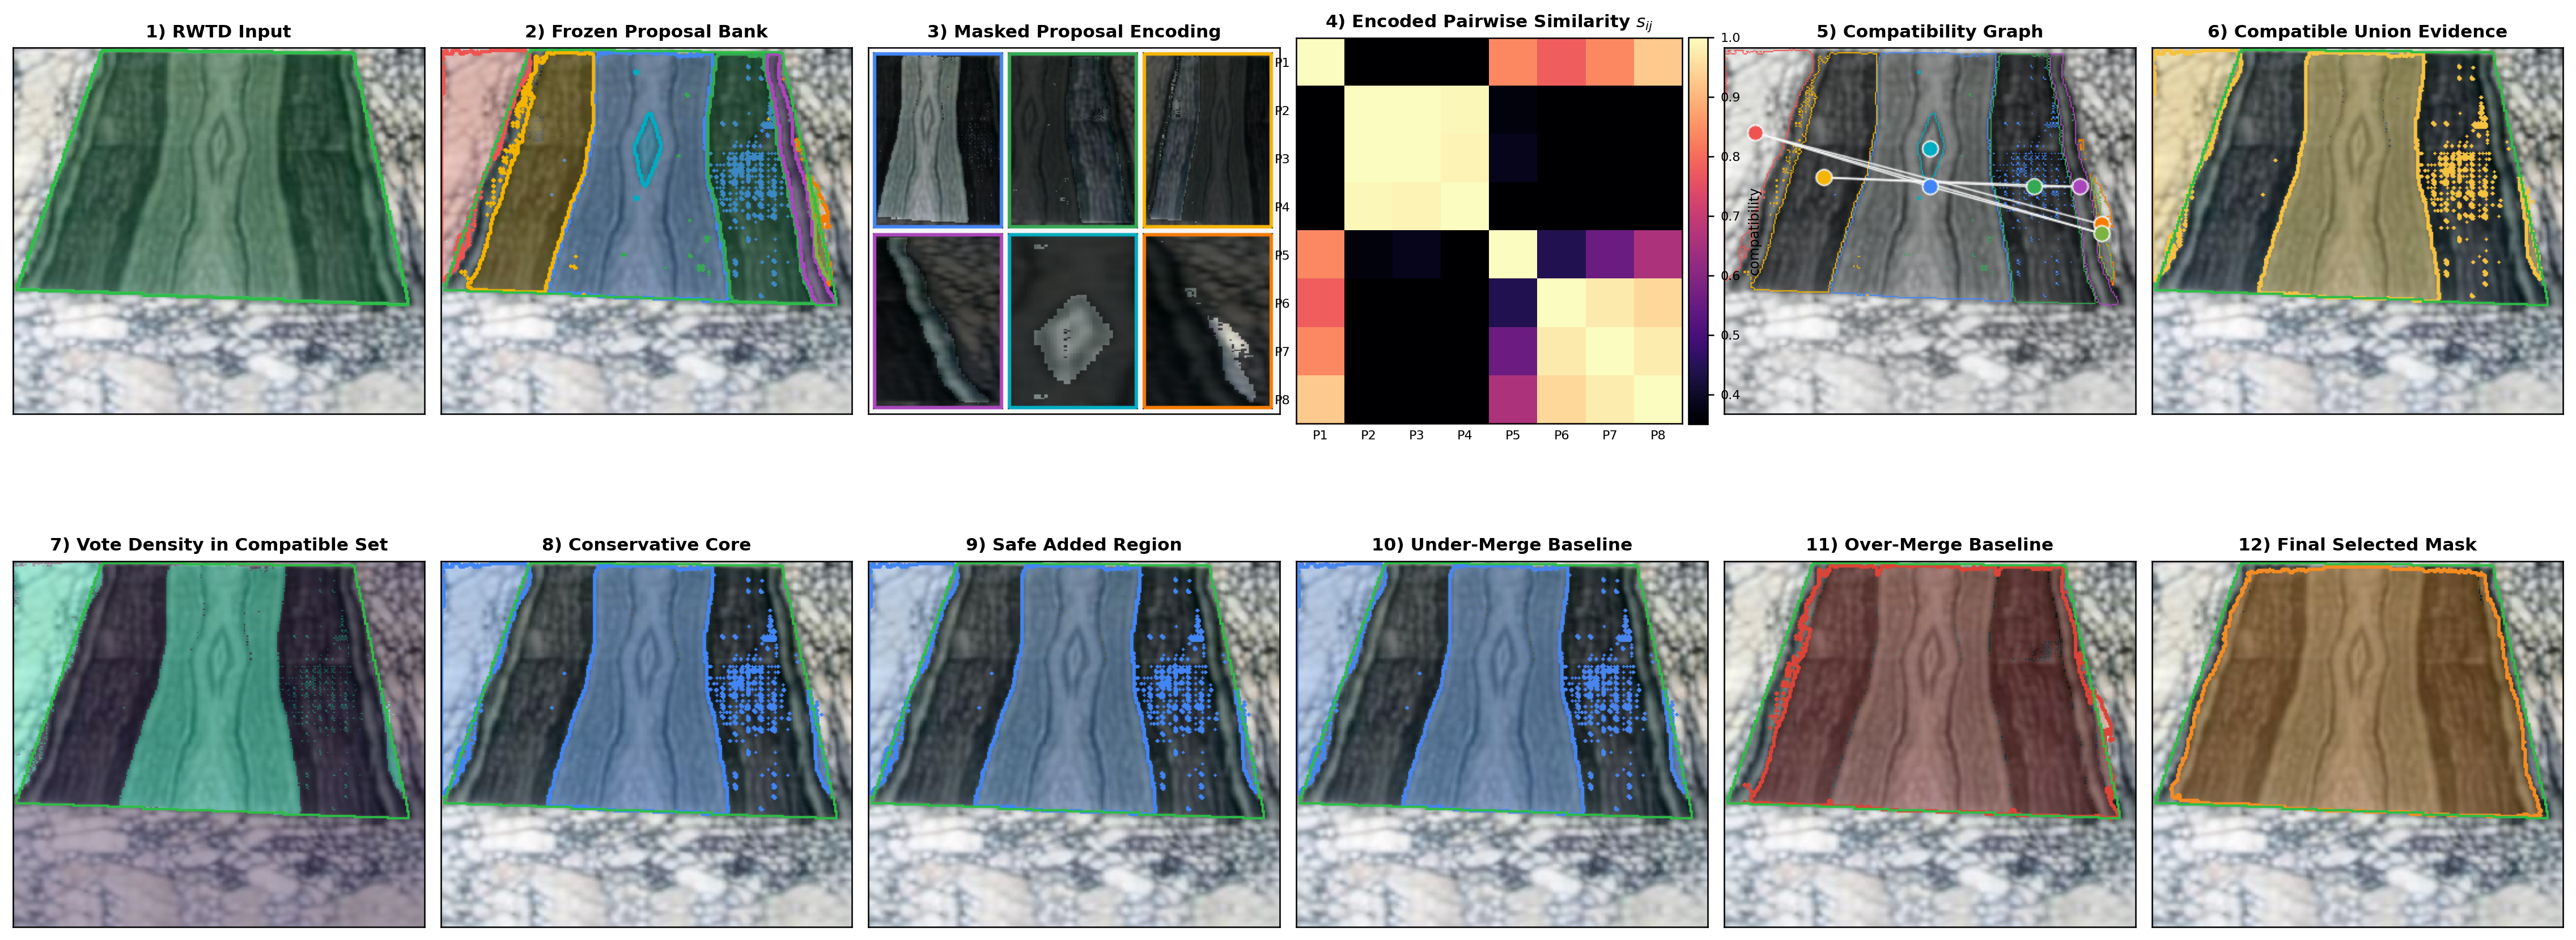
\includegraphics[width=0.98\textwidth]{figures/fig_consolidation_logic.png}
    \caption{Proposal-/mask-space exploration in implementation form. Each frozen proposal $m_i$ is encoded as a hybrid texture descriptor $d_i$, a learned pair model merges compatible proposals into candidate components, a learned component scorer selects a conservative core $C^\star$, and on RWTD only a learned dense-rescue switch can replace $C^\star$ with a denser candidate. Relative to the feature-space route, this figure answers a different question: not what the frozen representation contains internally, but what can already be recovered from the generated mask bank itself.}
    \label{fig:proposal_logic}
\end{figure*}

The implementation makes the learned objects explicit. Each proposal $m_i$ is encoded by a hybrid descriptor
\begin{align}
d_i = [h_i ; e_i],
\end{align}
where $h_i$ is a 60-D handcrafted summary of a 15-channel training-free texture map and $e_i$ is a PTD descriptor built from a masked crop plus ring context. The PTD encoder produces a 512-D region embedding, a second 512-D ring-context contrast term, and concatenates them into a 1024-D descriptor. The handcrafted map concatenates LAB color, Sobel $x/y/\|\nabla\|$, a Laplacian response, and an 8-filter Gabor bank; $h_i$ stores the mean, standard deviation, lower quartile, and upper quartile of those channels inside the proposal mask. Stage-A therefore uses a 1084-D descriptor per proposal.

Proposal compatibility is learned with a \textsc{RandomForestClassifier} over a 10-D pair feature vector. That vector includes descriptor cosine similarity, proposal area ratios, pair IoU, near-contact statistics, weak-boundary evidence, texture heterogeneity of the union, centroid distance, and union area ratio. Positive pair labels come from PTD-synthetic compositions: two proposals are compatible only when they cover the same synthetic texture region with sufficient purity. Thresholding these pair scores produces a compatibility graph, and its connected components define the candidate merged regions.

Candidate components are then ranked by a \textsc{RandomForestRegressor} over a second 10-D feature vector. Those component features include region area ratio, inside-versus-outside texture contrast, within-region variance, fragmentation penalty, boundary strength, compactness, descriptor variance within the component, descriptor separation from the complement, and proposal-count statistics. The regressor is trained to predict candidate IoU against the synthetic ground-truth partition, and the highest-scoring candidate becomes the conservative core $C^\star$.

RWTD adds one more learned decision layer above that core. A denser auxiliary bank proposes rescue candidates $R_k$ around under-covered scenes. For each $(C^\star, R_k)$ pair, the RWTD rescue path builds a core-versus-candidate feature vector that includes predicted score gaps, relative area and overlap, proposal-union coverage and precision, texture contrast, variance, and fragmentation deltas. A balanced logistic classifier predicts whether switching to $R_k$ is a safe positive move under \texttt{oracle\_safe\_winner} labels, and a \textsc{HistGradientBoostingRegressor} predicts the expected gain. The deployed \texttt{candidate\_cls} rule keeps the core unless some rescue candidate is classified positive, in which case it selects the positive candidate with highest predicted gain. STLD and the appendix routes stop at Stage-A and never invoke this rescue layer.
In notation,
\begin{align}
p_{\mathrm{safe}}(k) &= f_{\mathrm{safe}}(u(C^\star, R_k)),\\
g_{\mathrm{gain}}(k) &= f_{\mathrm{gain}}(u(C^\star, R_k)),
\end{align}
where $u(C^\star, R_k)$ is the rescue feature vector. The deployed prediction is
\begin{align}
\hat{Y}_{\mathrm{prop}} =
\begin{cases}
R_{k^\star}, & \exists k : p_{\mathrm{safe}}(k) > \tau_{\mathrm{safe}}, \; k^\star = \arg\max_{k: p_{\mathrm{safe}}(k) > \tau_{\mathrm{safe}}} g_{\mathrm{gain}}(k),\\
C^\star, & \text{otherwise.}
\end{cases}
\end{align}

\paragraph{Training regime and frozen components.} The proposal generator is frozen. This route does not retrain SAM, alter the prompt source, or optimize the bank with RWTD labels. What is learned instead is the decision stack above the bank. The RWTD Stage-A bundle used here is trained on 480 PTD-only synthetic samples, and the RWTD rescue bundle is trained on 256 PTD-only \texttt{repair\_mix} samples that inject explicit under-coverage cores and hard wrong-side decoys. The STLD Stage-A bundle is trained on 1600 PTD-only MPEG7-shape synthetic layouts. This separation is why the route speaks directly to recoverability: it measures how much task value remains once proposal generation is treated as fixed evidence rather than as the object of adaptation.

\paragraph{Why this model family?} The readout is deliberately small. The goal of the paper is to inspect what the frozen mask bank already contains, not to bury that question inside a new end-to-end network. The available supervision is limited and synthetic, the proposal descriptors mix heterogeneous geometric and texture cues, and the RWTD rescue path must remain modular enough to turn on only where it is needed. Tree-based models fit that regime well: they combine mixed tabular signals robustly, remain easy to audit at the level of pair scores and candidate rankings, and let the proposal bank stay fixed throughout. Appendix~\ref{app:implementation_details} summarizes the deployed inference algorithm, descriptor ablations, and the resulting practicality profile.
